	Dans le but de répondre aux besoins explicités précedemment, j'ai décidé d'avoir recours à un gestionnaire de tests sous forme d'une application web. En effet, celle-ci pourrait être mise en place sur un seveur interne et rendue disponible pour toute l'équipe, favorisant ainsi le partage d'information et permettant de centraliser toutes les données concernant la réalisation des tests fonctionnels, assurant ainsi un versionning cohérent. De plus, cela répond à la problématique de mise en place rapide et de maintenabilité efficace (pas de mise à jour à gérer sur tous les postes, etc...). \\
	
	Après avoir mené plusieurs recherches, j'ai pu constater qu'il existait différents gestionnaires open-source concurrents sur le marché répondant à nos exigences : \textit{Salomé TMF}, \textit{TestLink} ou encore \textit{Squash TM}. En effet, ces derniers nous offrent tous la possibilité de créer des tests, de les lier aux exigences client ou encore de créer des campagnes de tests puis d'exporter les résultats sous forme de rapport détaillé. Ces outils proposant des fonctionnalités très proches, j'ai décidé d'en choisir un disposant d'une grande flexibilité ainsi que d'une communauté active afin de pouvoir faciliter l'adaptation à nos cas de tests. En effet, les gestionnaires génèrent des rapports regroupant des informations telles que la description des tests, leur temps d'exécution ou leur status. Cependant, dans notre cas, nous souhaitions pouvoir inclure pour chacun des tests des informations supplémentaires telles que le nom du service auquel appartient la fonctionnalité testée, l'identifiant de l'utilisateur utilisé pour le test, le numéro de compte bancaire utilisé et de manière générale, tous les paramètres utilisés pour réaliser la reqûetes testées. PBI partageant les mêmes données que nous sur les environnements d'homologatoin et de pré-production, il leur était alors possible de vérifier de leur côté que les tests passent effectivement. De plus, lorsqu'ils remarquaient une anomalie, ils pouvaient nous transmettre les paramètres qu'ils avaient utilisé afin que nous puissions reproduire celle-ci chez nous. \\
	
	Ainsi, j'ai décidé d'utiliser l'outil \textit{TestLink} dont la communauté avait mis à disposition de tous des templates permettant de modifier le code source afin de customiser la génération des rapports de tests. Celui-ci est une application web développée en PHP et utilisant le système de gestion de base de données MySQL. Il permet de centraliser toute la gestion des tests fonctionnels du projet en les organisant par le biais des structures présentées dans le tableau \ref{structuresTestlink}.
	
	\newpage

\begin{table}[h!]
	\center
	\begin{tabular}{| c | c |}
     \hline
     Cas de test & Test fonctionnel définissant un scénario spécifique \\ \hline
     Suite de tests & Collection de cas de test validant une même fonctionnalité \\ \hline
     Plan de tests & Collection de suite de tests contenant toutes les informations \\  & telles que la portée, les étapes, la version etc...\\ & Un plan est exécuté pour un build particulier \\ \hline
     Build & Une release spécifique des APIs testées \\
     \hline
	\end{tabular}
	\caption{Structures fournies par TestLink}
	\label{structuresTestlink}
\end{table}

Cet outil présente de nombreux avantages qui m'ont conforté dans mon choix :
\begin{itemize}
	\item Campagnes de tests versionnées dont l'historique est enregistré en base de données.
	\item Export et import de cas de test et de leur résultats
	\item Connection avec \textit{Mantis}, un tracker de bug utilisé dans notre projet
	\item Gestion de rôles sur les tests (qui effectues le test, qui valide etc...)
	\item Rapport complet dans différents formats
	\item Accessible à toute l'équipe n'importe quand 
	\item Simplicité d'utilisation et de mise en place \\
\end{itemize}

	Ensuite, avant de procéder à la création des cas de test sur TestLink, j'ai commencé par définir la structure du futur plan de test qui serait exécuté avant chaque livraison. Ainsi, j'ai décidé de séparer l'ensemble des tests en deux grandes familles : ceux concernant les fonctionnalités de consultation et ceux concernant les fonctionnalités de transaction, ce qui m'amena à la création de deux suites de tests. Après cela, j'ai créé autant de suites de tests qu'il y avait de fonctionnalités décrites dans l'annexe \ref{a2}. Il est possible d'observer sur la figure \ref{testlink} l'organisation d'un plan de test type. Afin de garder le même formalisme tout le long de la réalisation des plans de tests et pour assurer une certaine cohérence, j'ai décidé de mettre en place plusieurs conventions définissant une stratégie de test :
	
	\subsubsection*{Cas de test}
	Les cas de tests doivent avoir un nom de la forme [id]-[titre] où
	\begin{itemize}
		\item id désigne un ID unique permettant de les identifier rapidement et de faciliter leur organisation. Celui-ci est \textit{NOBC-API-XX}, où XX représente le numéro du test. 
		\item titre désigne de manière clair et concise l'objectif du test
	\end{itemize}		
	De plus, chaque cas de test possède en attribut un numéro de version de la forme \textit{vX} où X est incrémenter de 1 chaque fois que le cas de test est modifié.
	
	\subsubsection*{Plan de test}
	Les plans de tests doivent avoir un nom de la forme [scope]-[environnement]-[version] où
	\begin{itemize}
		\item scope désigne la portée du plan de test : "complete" pour tous les tests, "transaction service" pour les tests du service de transaction, "transaction overview" pour les tests de la fonctionnalité transaction overview etc...
		\item environnement désigne le serveur sur lequel sont effectués les tests : homo3 ou rgb
		\item version est de la forme vX.Y.Z où
			\begin{itemize}
				\item X est incrémenté de 1 lorsqu'un nouveau cas de test est ajouté ou supprimé du plan
				\item Y est incrémenté de 1 lorsqu'un cas de test existant du plan a été modifié
				\item Z est incrémenté de 1 à chaque exécution du plan
			\end{itemize}
	\end{itemize}
	
	\subsubsection*{Build}
	Les builds doivent avoir un nom de la forme : [version] où
	\begin{itemize}
		\item version désigne la version de l'API microservices testée \\
	\end{itemize}

	La stratégie de test étant définie, il fallait maintenant déterminer quelles informations devaient être transmises au sein des rapports de tests. Les gestionnaires de tests proposent de remplir des formulaires afin consigner le résultat des tests une fois ceux-ci effectués, ce qui servira par la suite à générer un rapport. Cependant, ces derniers sont plutôt génériques et ne permettent pas de renseigner des données spécifiques à un projet particulier. Comme nous l'avons dit plus haut, nous souhaitions être en mesure de passer des paramètres supplémentaires afin de faciliter nos échanges avec PBI, comme : \\
	
	\begin{itemize}
		\item url et paramètres utilisés pour la requête
		\item service testé
		\item identifiants utilisés
	\end{itemize}
	
	\begin{figure}[h!]
	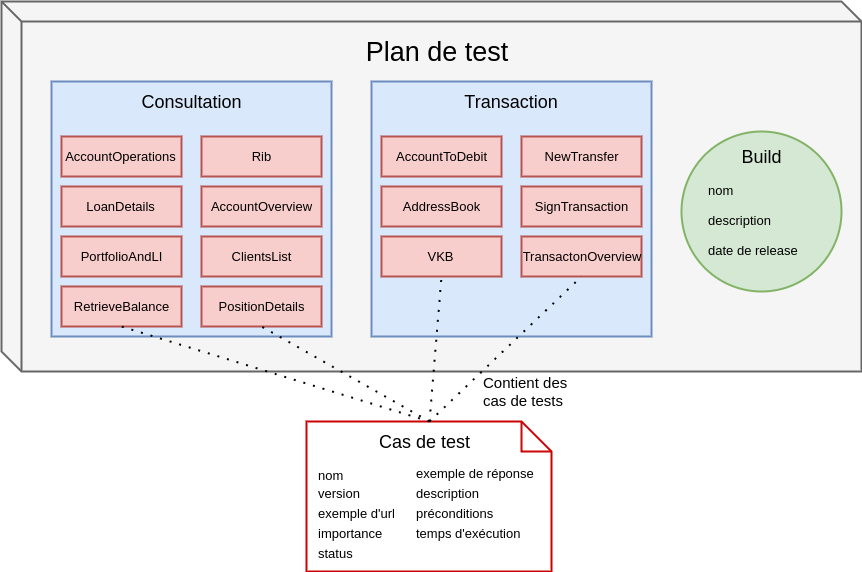
\includegraphics[scale=0.5]{images/travailNeuflizeOBC/architecture/testlink.png}
	\centering
	\caption{Configuration d'un plan de test type}
	\label{testlink}
\end{figure}
	
	Ainsi, j'ai décidé de modifier le code source de TestLink afin de rajouter les champs dont nous avions besoin aux formulaires de tests. J'ai réalisé cette modification en deux étapes dont la première consistait à ajouter les champs aux formulaires puis à gérer la partie front en PHP. La seconde concernait la récupération des données et leur sauvegarde en base de données, ce qui a impliqué la création de nouvelles requêtes SQL. Une fois les champs mis en place, j'ai créé un cas de test puis générer un premier rapport au format PDF en guide de POC (proof of concept). Celui-ci ayant été jugé satisfaisant, j'ai dû étudier l'ensemble des spécifications du projet concernant chacun des services mis en place afin de procéder à l'écriture de tous les cas de tests. Cela m'a permis de mieux comprendre le besoin du client, d'avoir une bien meilleure vision sur le projet dans sa globalité en m'apportant des informations sur l'utilité de chaque service et de pouvoir me former sur le projet en restant productif.
	
	Ces cas de tests permettaient de vérifier que les réponses des requêtes émises vers l'API microservices étaient en accord avec les attentes de PBI. Par exemple, les réponses étant au format JSON, ils permettaient la vérification de la présence de tous les champs obligatoires, la cohérence des valeurs des champs (\hl{TODO exemple a prendre dans la spec}) ou encore la vérification de la cohérence des données de notre backend avec celles de l'application web.